\section{Zielsetzung}
In diesem Versuch werden die Suszeptibilitäten von seltenen Erden untersucht, sowie die Filterkurve des Selektivverstärkers, welcher im Versuch benutzt wird.

\section{Theoretische Grundlagen}
Allgemein kann die magnetische Flussdichte $\symbf{B}$ mit der magnetischen Feldstärke $\symbf{H}$ und der Magnetisierung $\symbf{M}$ angegeben werden als
\begin{equation}
        \vec B = \mu_0 \vec H + \vec M \, ,
    \label{eqn:b}
\end{equation}

\noindent
wobei die Magnetisierung $\symbf{M}$ ebenfalls von der magnetischen Feldstärke $\symbf{H}$ abhängt, sodass 

\begin{equation}
        \label{eqn:m}
        \vec B = \mu_0 \vec H + \mu_0 \chi \vec H 
\end{equation}

\noindent
gilt. Dabei ist die magnetische Suszeptibilität $\chi$ eine dimensionslose Größe, die angibt, wie gut ein Material im externen Magnetfeld magnetisierbar ist. 
Im Allgemeinen wird zwischen zwei Arten von Magnetisierungen unterschieden. Zum einen in Stoffen welche diamagnetisch sind, also Stoffe bei der  $\chi < 0$ ist 
und somit bei einem Feld, welches von außen anliegt, dem entgegengesetzt zur Feldrichtung magnetisiert werden. 

\noindent
Zum anderen in Stoffe, welche die Eigenschaft der Suszeptibilität besitzen, also bei denen $\chi > 0$ ist. Diese Eigenschaft wird nur bei Stoffen beobachtet,
welche einen nicht verschwindenden Drehimpuls haben. Bei diesen Materialien gilt ein antiporpotionales Verhältnis der 
Suszeptibilität zur Temperatur. 

\begin{equation}
        \chi \propto \frac{1}{T}
\end{equation}

\noindent
Dies wird auch das Curiesche Gesetz genannt. 

\noindent
Bei Seltenen-Erd-Verbindungen kommt der Gesamtdrehimpuls durch die Anordnung der 4f-Elekronen Zustande.
Für diese Elektronen und den Gesamtdrehimpuls $\vec{J}$ gelten die Hundschen Regeln:

\begin{itemize}
    \item Die einzelnen Spins $\vec{s_i}$ summieren sich nach dem Pauli-Prinzip zum maximalen Gesamtspin
    $\vec{S} = \sum \vec{s_i}$ auf.
    \item Die einzelnen Bahndrehimpulse $\vec{l_i}$ summieren sich nach dem Pauli-Prinzip zum Maximaldrehimpuls 
    $\vec{L} = \sum \vec{l_i}$ auf.
    \item Der Gesamtdrehimpuls beträgt $\vec{J} = \vec{L} - \vec{S}$, wenn die Elektronenschale weniger und
    $\vec{J} = \vec{L} + \vec{S}$, wenn die Schale mehr als halbvoll besetzt ist.
\end{itemize}

\noindent
Allgemein ist der quantenmechanische Zusammenhang zwischen Drehimpuls und dem magnetischen Moment geben durch:

\begin{align}
        \vec{\mu_\text{L}} &= - \frac{\mu_\text{B}}{\hbar} \vec{L} \; , \\
        \vec{\mu_\text{S}} &= - g_\text{S} \frac{\mu_\text{B}}{\hbar} \vec{S} \, ,
\end{align}

\noindent
wobei $\mu_\text{B}=\frac{\hbar e_0}{2m_0} $ das Bohrsche Magneton und $g_\text{S}$ das gyromagnetische Verhältnis beschreibt.

\noindent
Dabei setzt sich der Drehimpuls $\vec{J}$ aus dem Bahndrehimpuls der Elektronenhülle $\vec{L}$ und dem Gesamtspin $\vec{S}$ zusammen. Eigentlich müsste der Kerndrehimpuls mitbetrachtet
werden, jedoch kann er an dieser Stelle vernachlässigt werden.

\begin{figure} [H]
        \centering
        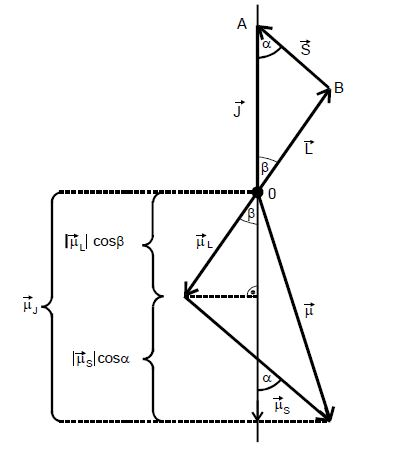
\includegraphics[scale=0.75]{Bilder/Vek.JPG}
        \caption{Vektordiagramm aus den Drehimpulsvektoren einer Elektronenhülle. \cite{V606}}
        \label{fig:plot3}
\end{figure}

\noindent
Damit ergibt sich mit den Quantenzahlen der Drehimpulse $\vec{J}$ und $\vec{L}$ und des Spins $\vec{S}$ die Beträge

\begin{equation*}
        |\vec{\mu_\text{J}}| = |\vec{\mu_\text{S}}| \cdot \text{cos}\left(\alpha \right) + 
        |\vec{\mu_\text{L}}| \cdot \text{cos}\left(\beta \right) \, .
\end{equation*}

\noindent
Zusätzlich lässt sich daraus und der \autoref{fig:plot3} der Lande-Faktor bestimmen zu

\begin{equation*}
        g_J = \frac{3J(J+1) + [S(S+1) - L(L+1)]} {2 J(J+1)} \, .
        \label{eqn:lande}
\end{equation*}

\noindent
Daraus folgt für $|\vec{\mu_\text{J}}|$:

\begin{equation}
    |\vec{\mu_\text{J}}| = \vec{\mu_\text{B}} g_J \sqrt{J (J+1)}  \, .
\end{equation}

\noindent
Aus der Quantenmechanik geht zusätzlich noch eine Richtungsquantelung vor. Das bedeutet, dass der Winkel zwischen dem äußeren Magnetfeld und dem $\vec{\mu_\text{J}}$
nicht kontinuierlich ist, sondern nur diskrete Werte annehmen kann. Und zwar nur die Werte (am Beispiel der Z-Komponente), bei denen 
\begin{equation}
        \mu_{J_Z} = - \mu_\text{B} \cdot g_J \cdot m
\end{equation}

\noindent
gilt, wobei $m$ die ganzzahlige Orientierungsquantenzahl ist und durch die es $2J+1$ Einstellungsmöglichkeiten bezüglich des äußeren Magnetfeldes gibt. Daraus kann allgemein der
Zusammenhang 
\begin{equation}
        \chi = \frac{\mu_0 \cdot \mu_\text{B}^2 \cdot g_J^2 \cdot N J (J+1)}{3kT}
        \label{eqn:theo}
\end{equation}

\noindent
geschlussfolgert werden.

\noindent
Wird in eine Spule ein Stoff mit paramagnetische Suszeptibilität eingeführt und dann mit einer Spule verglichen, in welcher kein Stoff ist, so fällt ein eine Induktivitätsdifferenz
$\Delta L$ zwischen den Spulen auf. Dieser Unterschied wird genutzt um Stoffe mit paramagnetischer Suszeptibilität mit einer Brückenschaltung zu untersuchen.
Dabei wird diese aufgebaut wie in \autoref{fig:bruecke} dargestellt.

\begin{figure}[H]
        \centering
        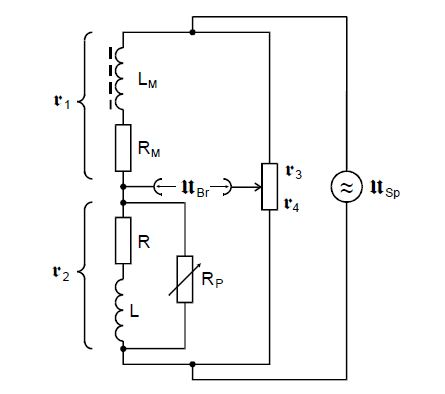
\includegraphics[width=0.75\textwidth]{Bilder/MessBruecke.JPG}
        \caption{Brückenschaltung zur Suszeptibilitätsmessung \cite{V606}.}
        \label{fig:bruecke}
\end{figure}

\noindent
Für für hohe Spannungsfrequenzen kann aus der Abbildung geschlossen werden, dass für $\omega^2 L^2 >> R^2$ die Beziehung 
\begin{equation}
    \chi (\omega \to \infty) = \frac{4 F U_\text{Br}}{Q U_\text{Sp}} 
    \label{eqn:spannung}
\end{equation}

\noindent 
gilt. Dabei ist  $F$ der Spulenquerschnitt, $Q$ der Probenquerschnitt und $U_\text{Sp}$ die Speisespannung.

\noindent
Zusätzlich kann die Methode mit erneutem Abgleich der Brückenspannung die Beziehung 
\begin{equation}
    \chi = \frac{2 \cdot \Delta R \cdot F}{R_3\cdot Q}
    \label{eqn:alternativ}
\end{equation}

\noindent
benutzt werden, wobei $\Delta R$ für die Differenz der Potentiometereinstellungen steht.

\noindent
Bei der Messung mit der Brückenspannung treten jedoch Störspannungen auf, welche mit einem Selektivverstärker deutlich verringert werden können. 
\begin{figure}[H]
        \centering
        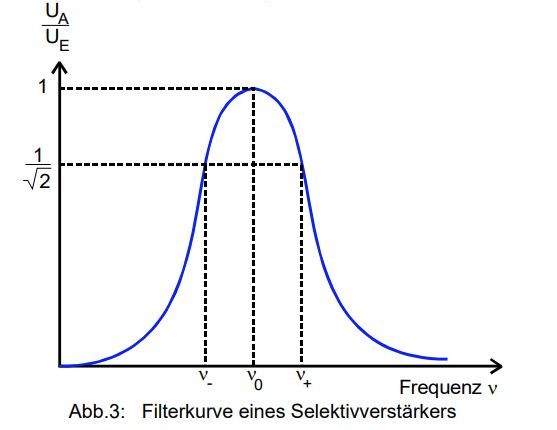
\includegraphics[width=0.75\textwidth]{Bilder/Kurve.jpg}
        \caption{Filterkurve \cite{V606}.}
        \label{fig:filterkurve2}
\end{figure}

\noindent
Dabei gibt die Güte $Q$ die Qualität des Filters an. Je Spitzer die Kurve ist, je höher ist die Güte und die Qualität des Filters. Diese kann berechnet werden mit 
\begin{equation}
        \label{eqn:güte}
        Q = \frac{\nu_0}{\nu_+ - \nu_-} \, ,
\end{equation}

\noindent
wobei $\nu_0$ die Durchlassfrequenz des Selektivverstärkers ist und $\nu_+$ und $\nu_-$ die Frequenzen, bei denen $\frac{U_\text{A}}{U_\text{E}}$ den Wert $\frac{1}{\sqrt{2}}$ erreicht.

